\problemname{Cakes and Ogres
}

\intextsep2mm
\begin{wrapfigure}{r}{50mm}
 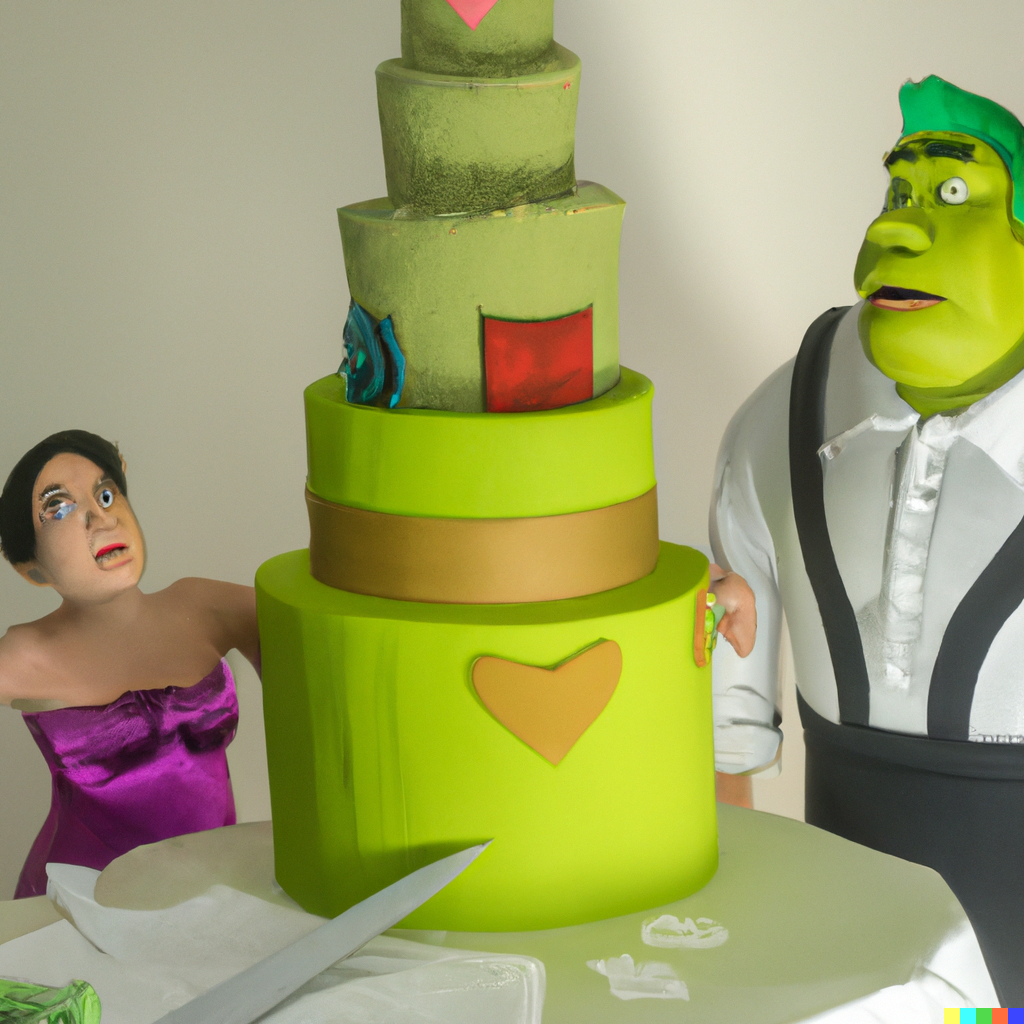
\includegraphics[width=50mm]{img.png}
\end{wrapfigure}
~

Cakes and Ogres are alike in one important way: They both have layers.

Fiona is planning her wedding and is trying to assemble a delicious cake out of a collection of possible cake layers. Each layer has a weight, a carrying capacity, and a deliciousness. Layers can be stacked on top of one another in any order to create the cake. The cake will collapse if the carrying capacity of a layer is lower than the sum of the weight of that layer plus all the weights of the layers above that layer. That is, a layer must carry itself and all the layers above it.

Fiona wants to maximise the sum of deliciousness values for the layers in the cake such that the cake does not collapse.


\section*{Input}

The first line of input contains the integer $N$~($1 \leq N \leq 10$), the number of layers.

The next $N$ lines describe the layers. The $i$th of these lines contains three integers $W_i$~($1 \leq W_i \leq 10^9$), $C_i$~($W \leq C_i \leq 10^9$), and $D_i$~($1 \leq D_i \leq 10^9$), which are the weight, carrying capacity, and deliciousness of the $i$th layer respectively.


\section*{Output}

Display the maximum sum of deliciousness values.

